\documentclass[11pt]{article}
\usepackage{fullpage,amsmath,amsfonts,mathpazo,microtype,nicefrac,graphicx}

% Set-up for hypertext references
\usepackage{hyperref,color,textcomp}
\definecolor{webgreen}{rgb}{0,.35,0}
\definecolor{webbrown}{rgb}{.6,0,0}
\definecolor{RoyalBlue}{rgb}{0,0,0.9}
\hypersetup{
   colorlinks=true, linktocpage=true, pdfstartpage=3, pdfstartview=FitV,
   breaklinks=true, pdfpagemode=UseNone, pageanchor=true, pdfpagemode=UseOutlines,
   plainpages=false, bookmarksnumbered, bookmarksopen=true, bookmarksopenlevel=1,
   hypertexnames=true, pdfhighlight=/O,
   urlcolor=webbrown, linkcolor=RoyalBlue, citecolor=webgreen,
   pdfauthor={Chris H. Rycroft},
   pdfsubject={Harvard AM205 (Fall 2017)},
   pdfkeywords={},
   pdfcreator={pdfLaTeX},
   pdfproducer={LaTeX with hyperref}
}
\hypersetup{pdftitle={AM205: Final Project}}

% Macro definitions
\newcommand{\N}{\mathbb{N}}
\newcommand{\Z}{\mathbb{Z}}
\newcommand{\Q}{\mathbb{Q}}
\newcommand{\R}{\mathbb{R}}
\newcommand{\B}{\mathbb{B}}
\newcommand{\mcL}{\mathcal{L}}
\newcommand{\p}{\partial}
\newcommand{\Trans}{\mathsf{T}}
\renewcommand{\vec}[1]{\mathbf{#1}}
\newcommand{\vx}{\vec{x}}
\newcommand{\vb}{\vec{b}}

\DeclareMathOperator{\rank}{rank}

\begin{document}
\section{Results and Discussions}
\subsection{Simple ODEs}
Overview

Consider a first-order ODE system:
    \begin{equation}
      \frac{dx}{dt} = \cos t+x^2 + y - (1 + t^2 +\sin^2t)
      \label{eq:simple_eq1}
    \end{equation}
    
     \begin{equation}
      \frac{dy}{dt} = 2t - (1 + t^2)\sin t + xy
      \label{eq:simple_eq2}
    \end{equation}

    
where $t \in [0, 3]$.

Mathematics

The analytical solutions are:
    \begin{equation}
      x = \sin t
      \label{eq:simple_eq3}
    \end{equation}
    
     \begin{equation}
      y= 1 + x^2
      \label{eq:simple_eq4}
    \end{equation}

Results 

The solutions using the Neural Net solver could be found in Fig.~\ref{fig:SimpleFig}. The network was trained using a grid of 20 equidistant points in $t = [0, 3]$ and 50 hidden units in the hiddlen layer. 

We could see an almost exact fit with the analytical solution. In terms of training convergence, we could see that the neural net rapidly converges to the solution with just a few iterations from Fig. ~\ref{fig:SimpleLoss}.

To enable us to evaluate the fit of the two functions in this system of ODE, we propose taking an average of the RMSE, in this case we will have:

\begin{equation}
RMSE_{overall} = \frac{1}{2}[RMSE_{x} + RMSE_{y}]
\end{equation}

The fitting attained as shown in Fig. \ref{fig:SimpleFig} has $RMSE_{overall} = 0.0177$

Note that average RMSE enables us to determine the reproducibility of a good performing model for the same ODE system, which is discussed in the next section. 

\begin{figure}
\centering
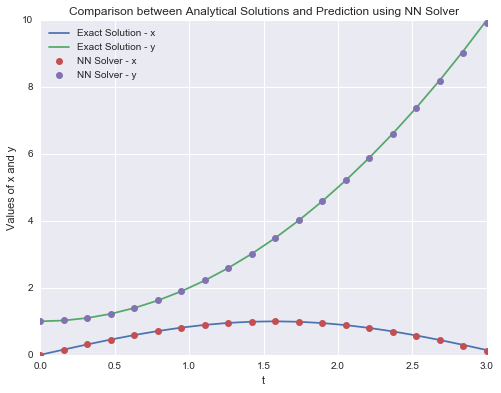
\includegraphics[width=0.7\textwidth]{result_simple.png}
      \caption{Comparing solutions found using neural net solver versus exact analytical solutions.\label{fig:SimpleFig}}
\end{figure}

\begin{figure}
\centering
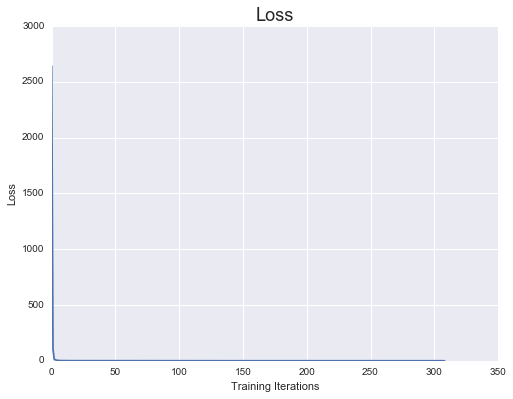
\includegraphics[width=0.7\textwidth]{loss_simple.png}
      \caption{Convergence to final solution. \label{fig:SimpleLoss}}
\end{figure}

Discussions

In terms of reproducibility, we repeated the same fitting process 100 times. The average RMSE histogram distribution for 100 fittings is shown in Fig. \ref{fig:SimpleHistogram}. 67\% of the fittings are relatively close fit to the exact analytical solution.

\begin{figure}
\centering
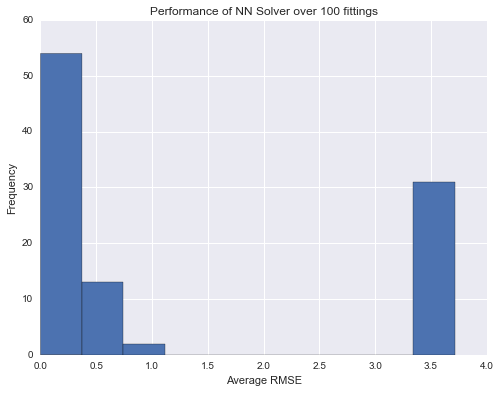
\includegraphics[width=0.7\textwidth]{histogram_simple.png}
      \caption{Average RMSE Distribution for 100 Repeated Fittings \label{fig:SimpleHistogram}}
\end{figure}

The model does not perform as well in extrapolation. As shown in Fig. \ref{fig:SimpleExtrap}, the fitting is accurate only up to $t = 3.5$, i.e. $0.5$ unit of time beyond the maximum time point in training. 

\begin{figure}
\centering
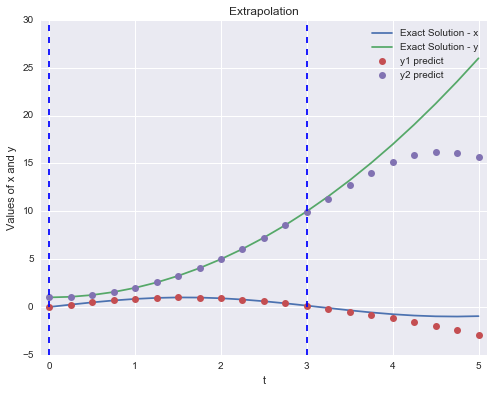
\includegraphics[width=0.7\textwidth]{extrapo_simple.png}
      \caption{Extrapolation: Predicting on values beyond $t\in [0, 3]$ \label{fig:SimpleExtrap}}
\end{figure}


\subsection{Unstable, Periodic ODEs}


\subsubsection{Lotka-Volterra 2-species model}
Overview
\break

The Lotka-Volterra prey-predator equations are a pair of first-order, non-linear differential equations commonly used to describe the interactions between two species, the prey and predator.
\break

Mathematics
\break
The populations of the prey and predator can be described by the following equations:

    \begin{equation}
      \frac{dx}{dt} = ax - bxy
      \label{eq:LV1}
    \end{equation}
    
     \begin{equation}
      \frac{dy}{dt} = -cy + dxy
      \label{eq:LV2}
    \end{equation}
    

where
\begin{itemize}
\item $x$ is the density of prey
\item $y$ is the density predator
\item $t$ represents time
\item $a, b, c, d >0$ 
\end{itemize}

Eq.~\ref{eq:LV1} indicates that in the absence of a predator ($y = 0$), the prey would grow at a constant rate $a$, with the assumption that the prey have an unlimited food supply. The rate of predation upon the prey is assumed to be proportional to the rate at which the predators and the prey are present concurrently, represented by $bxy$. If either $x$ or $y$ is zero then no predation is possible.

Similarly, Eq.~\ref{eq:LV2} shows that in the absence of prey ($x = 0$), the density of predators would decrease at a constant rate $c$, due to natural death or emigration. This equation assumes that the predator population only preys upon the same species of prey identified in Eq.~\ref{eq:LV1}. $dxy$ represents the growth of the predator population[REF1].

The model assumes that throughout the process the external environment remains the same and none of the species is favored.[REF2]

Results 
\break

\begin{figure}
\centering
\includegraphics[width=0.7\textwidth]{LV_compare.png}
      \caption{Comparing across results using standard ODE solver from Scipy library versus using neural net solver, at initial parameters of $a = 1$, $b = 0.1, c = 1.5, d = 0.75$. Average RMSE = 1.568. \label{fig:LVFig}}
\end{figure}

\begin{figure}
\centering
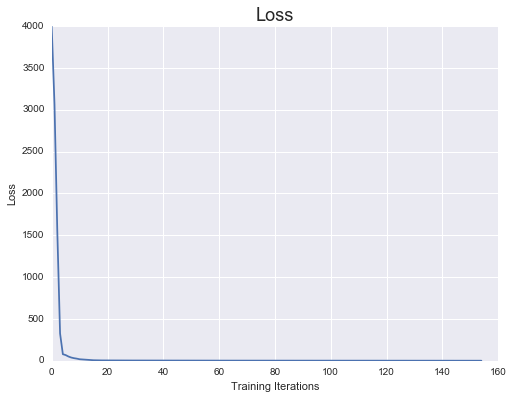
\includegraphics[width=0.7\textwidth]{loss_LV2.png}
      \caption{Convergence to final solutions for 2-species model \label{fig:loss_LV2}}
\end{figure}

From Fig.\ref{fig:LVFig} we see that our neural net solver attains a close fit to the ODE solver. Training was done with a grid of 100 equidistant points in $t = [0, 10]$ and 50 hidden units in the hidden layer. 

In terms of training convergence, we could see that the neural net rapidly converges to the solution with just a few iterations from Fig. ~\ref{fig:loss_LV2}.


The same as before, to enable us to evaluate the fit of the two functions in this system of ODEs, we propose taking an average of the RMSE, in this case we will have:

\begin{equation}
RMSE_{overall} = \frac{1}{2}[RMSE_{prey} + RMSE_{predator}]
\end{equation}

For this particular plot, the overall average RMSE is at $1.568$. It is found that while our proposed solver using neural net is able to provide a continuous function, the results tend to fluctuate highly. As such, we ran the same fitting over 100 times as shown in Fig. ~\ref{fig:perf_dist}. 30\% of the fittings result in relatively good fitting with average RMSE of less than 5.

\begin{figure}
\centering
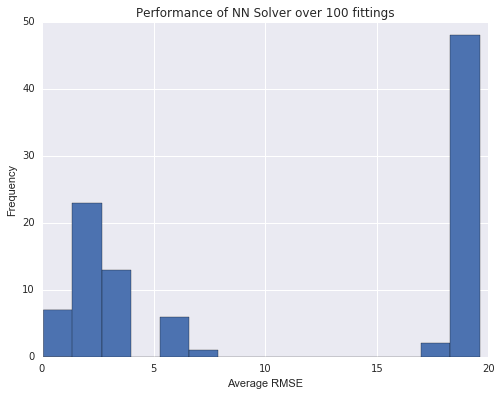
\includegraphics[width=0.7\textwidth]{perf_distribution.png}
      \caption{Running NN solver 100 times to see the performance histogram \label{fig:perf_dist}}
\end{figure}

Similar to the simple ODE system earlier, neural net model also does not perform well in extrapolation. We see from Fig.~\ref{fig:LV2Extrap} that the values deviate from the predicted values using ODE solver strongly beyond $t = 10$.

\begin{figure}
\centering
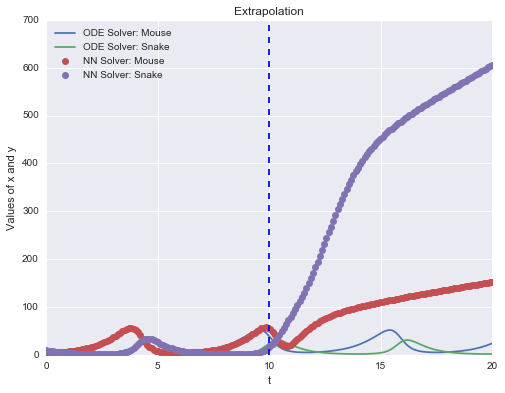
\includegraphics[width=0.7\textwidth]{extrapo_LV2.png}
      \caption{Extrapolation - Predicting on values beyond $t\in [0, 10]$ \label{fig:LV2Extrap}}
\end{figure}

\subsubsection{Lotka-Volterra 3-species Model}
Extending to the 2-species model discussed earlier, we wish to model a linear three-species food chain where the lowest-level prey $x$ is preyed upon by a mid-level species $y$, which, in turn, is preyed upon by a top level predator $z$. An example of a three-species food chain is mouse-snake-owl [REF3].  

    \begin{equation}
      \frac{dx}{dt} = ax - bxy
      \label{eq:LV3}
    \end{equation}
    
     \begin{equation}
      \frac{dy}{dt} = - cy + dxy - eyz
      \label{eq:LV4}
    \end{equation}
    
     \begin{equation}
      \frac{dz}{dt} = - fz + gyz
      \label{eq:LV5}
    \end{equation}
where
\begin{itemize}
\item $a, b, c, d, e, f, g >0$ 
\item $a, b, c, d$ are as in the 2-species Lotka-Volterra equations
\item $e$ represents the effect of predation on species $y$ by species $z$
\item $f$ represents the natural death rate of species $z$ in the absence of prey
\item $g$ represents the reproduction rate of species $z$ in the presence of prey $y$
\end{itemize}

Results
\begin{figure}
\centering
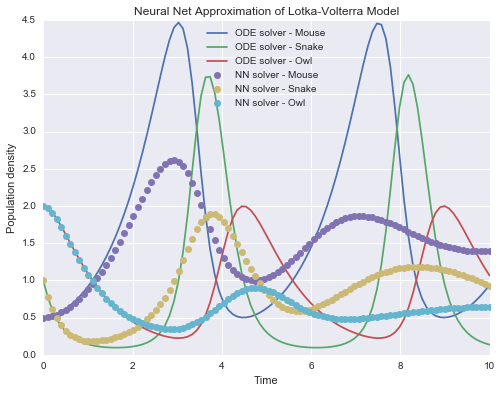
\includegraphics[width=0.7\textwidth]{LV_Compare_3_species.png}
      \caption{Comparing across results using standard ODE solver from Scipy library versus using neural net solver, at initial parameters of $a = b = c = d = e = f = g = 1 $. Average RMSE score of 0.803. \label{fig:LVFig_3_species}}
\end{figure}

The neutral net is trained with 50 hidden units over 100 equidistant points over $t \in [0, 10]$. From Fig.~\ref{fig:LVFig_3_species}, we can see that the performance is worse compared to the 2-species Lotka-Volterra model. The fit is close to the solution from ODE solver only up to $t = 1$ for the three equations. No further model fitting is carried out as the fitting is poor and the average RMSE score is not a good gauge to identify strong fit. 

In terms of extrapolating beyond the time range which the neural net was trained, the performance was not satisfactory. From Fig.~\ref{fig:LV3Extrap}, we see strong deviation from the ODE solver solution.


\begin{figure}
\centering
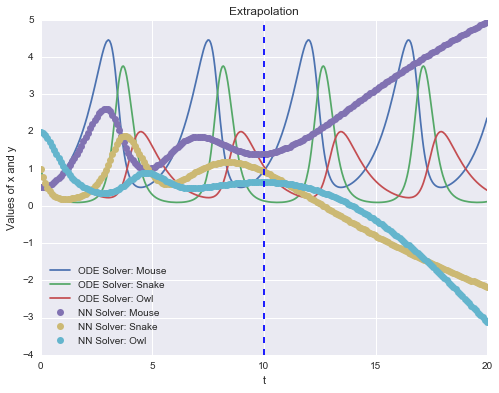
\includegraphics[width=0.7\textwidth]{extrapo_LV3.png}
      \caption{Predicting on values beyond $t\in [0, 10]$ \label{fig:LV3Extrap}}
\end{figure}


\subsubsection{Van der Pol oscillator}
Overview

Van der Pol oscillator is a non-conservative oscillator with a linear spring force and a non-linear damping force.  [REF4] The equation is given by:
     \begin{equation}
      \frac{d^2x}{dt^2} - \mu(1-x^2)\frac{dx}{dt} + x = 0
      \label{eq:VDP}
    \end{equation}
    
Mathematics

Applying the Li\'enard transformation $y = x - \frac{x^3}{3} - \frac{1}{\mu}\frac{dx}{dt}$, the equation can be written as a system of ODE [REF5]:

     \begin{equation}
      \frac{dx}{dt} = \mu(x - \frac{1}{3}x^3 - y)
      \label{eq:VDP1}
    \end{equation}
    
     \begin{equation}
      \frac{dy}{dt} = \frac{x}{\mu}
      \label{eq:VDP2}
    \end{equation}
    
Results

From Fig.\ref{fig:VDP_uniform} we see that our neural net solver attains a close fit to the ODE solver. Training was done with a grid of 40 equidistant points in $t = [0, 10]$ and 20 hidden units in the hidden layer. 

The same as before, to evaluate the fit of the two functions in this system of ODEs, we propose taking an average of the RMSE, in this case the overall average RMSE for our fit in Fig.~\ref{fig:VDP_uniform} is at $0.0135$. 

Since the fitting is satisfactory, we ran the same fitting over 100 times to ensure reproducibility. From Fig. ~\ref{fig:VDP_perf_dist}, 63\% of the fittings result in relatively good fitting with average RMSE of less than 2.5.

Similar to the simple ODE system earlier, neural net model also does not perform well in extrapolation. We see from Fig.~\ref{fig:VDP_extrapo} that the values deviate from the predicted values using ODE solver strongly beyond $t = 10$.

\begin{figure}
\centering
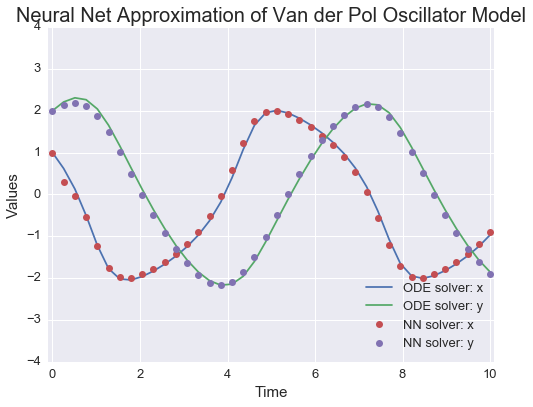
\includegraphics[width=0.7\textwidth]{VDP_uniform_good.png}
      \caption{Running NN solver with even spacing on time points. Average RMSE of 0.0135. \label{fig:VDP_uniform}}
\end{figure}


\begin{figure}
\centering
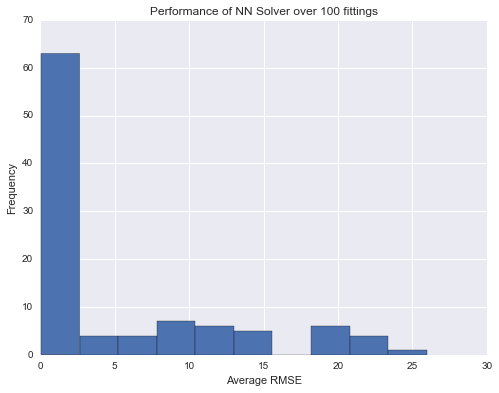
\includegraphics[width=0.7\textwidth]{VDP_DIst.png}
      \caption{Running NN solver 100 times to see the performance histogram \label{fig:VDP_perf_dist}}
\end{figure}

\begin{figure}
\centering
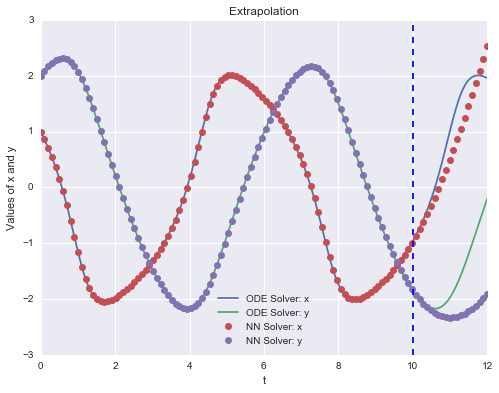
\includegraphics[width=0.7\textwidth]{extrapo_VDP.png}
      \caption{Running NN solver 100 times to see the performance histogram \label{fig:VDP_extrapo}}
\end{figure}


Discussions

63\% of the fittings attained average RMSE score of less than 2.63.


%1. https://en.wikipedia.org/wiki/Lotka-Volterra_equations
%2. http://www.math.harvard.edu/library/sternberg/slides/11809LV.pdf
%3. http://people.kzoo.edu/barth/math280/articles/3speciesLV.pdf
%4. http://www2.me.rochester.edu/courses/ME406/webexamp5/vanpol.pdf
%5. Kaplan, D. and Glass, L., Understanding Nonlinear Dynamics, Springer, 240–244, (1995).
\end{document}